\documentclass[12pt]{article}

%------------------------------------------------
% Fonts and layout
%------------------------------------------------
\usepackage{fontspec}
\setmainfont{TeX Gyre Pagella}

\usepackage{microtype}
\usepackage{geometry}
\geometry{margin=1in}

\usepackage{setspace}
\onehalfspacing

%------------------------------------------------
% Math and figures
%------------------------------------------------
\usepackage{amsmath}
\usepackage{amssymb}
\usepackage{amsthm}
\usepackage{graphicx}
\usepackage{caption}
\usepackage{booktabs}
\usepackage{array}
\usepackage{tabularx}
\usepackage{tikz}
\usetikzlibrary{calc,decorations.pathmorphing,shapes.geometric}
\usepackage{siunitx}
\usepackage{longtable}

%------------------------------------------------
% Bibliography and cross-references
%------------------------------------------------
\usepackage{natbib}
\bibliographystyle{apalike}

\usepackage{hyperref}
\hypersetup{colorlinks=true, linkcolor=black, citecolor=black, urlcolor=blue}

%------------------------------------------------
% Theorems / hypotheses
%------------------------------------------------
\newtheorem{hypothesis}{Hypothesis}
\newtheorem{prediction}[hypothesis]{Prediction}

%------------------------------------------------
% Title
%------------------------------------------------
\title{The Stone Piano Hypothesis:\\
Neanderthal Lithophones and the Acoustic Interpretation\\
of the Bruniquel Cave Structures}

\author{Flyxion}
\date{\today}

\begin{document}

\maketitle

\begin{abstract}
The circular stalagmite structures discovered deep within Bruniquel Cave (Tarn-et-Garonne, southwestern France) represent among the most enigmatic architectural constructions attributed to early \textit{Homo neanderthalensis}. Uranium--thorium dating places the construction of these features at approximately $176{,}500 \pm 2{,}100$ years before present \citep{Jaubert2016}, predating the arrival of anatomically modern humans in western Europe by more than one hundred thousand years and rendering Bruniquel the earliest known instance of deliberate subterranean construction in the hominin record. The assemblage comprises hundreds of intentionally fractured and repositioned stalagmites arranged in circular and semicircular formations approximately 336~m from the cave entrance, entirely beyond the penetration of natural light. Controlled fires were maintained within the chamber, and no habitation debris has been identified.

Existing interpretations have primarily framed the structures as architectural features of ritual or organizational significance without specifying a mechanism by which they would have functioned. The present paper proposes an alternative interpretive framework, designated the \textit{Stone Piano Hypothesis}, according to which the Bruniquel stalagmite assemblages functioned as lithophones: percussion instruments fabricated from resonant calcite speleothems capable of producing discrete tonal outputs when struck. On this reading, the Neanderthal builders intentionally selected, fractured, and arranged stalagmites so as to exploit the acoustic properties of calcite, transforming the deep-cave chamber into a resonant performative environment.

The hypothesis is motivated by converging lines of evidence: the mechanical and acoustic properties of calcite speleothems, the extensive ethnographic and archaeological record of lithophone use across Africa, Asia, and Europe, the growing body of archaeoacoustic research demonstrating systematic spatial relationships between resonance hotspots and prehistoric imagery, the unusual uniformity of stalagmite fragmentation at Bruniquel, the circular spatial organization of the rings, the subterranean context, and the complete absence of domestic occupation signatures. Although the hypothesis is at present speculative, it is formulated so as to be empirically testable through acoustic measurement of speleothem samples, morphometric analysis of fragment lengths, and digital modeling of chamber reverberation. The paper situates the hypothesis within broader debates concerning Neanderthal symbolic cognition, the deep evolutionary origins of musical behavior, and the epistemological standards appropriate to prehistoric archaeoacoustic interpretation.
\end{abstract}

\tableofcontents
\newpage

%=================================================================
\section{Introduction}
%=================================================================

The question of Neanderthal cognitive and cultural capacity has occupied paleoanthropology for over a century, and the terms of that debate have shifted substantially over the past two decades. Where earlier scholarship frequently characterized \textit{H.\ neanderthalensis} as cognitively conservative relative to anatomically modern humans, the accumulation of evidence for pigment use \citep{Zilhao2010, Roebroeks2012}, possible personal ornamentation \citep{Peresani2011, Radovčić2015, Morin2012}, dietary complexity \citep{Hardy2013}, fire management \citep{Sandgathe2011}, and independent regional technological traditions \citep{Wil2019} has produced a substantially revised picture. Neanderthals increasingly appear as behaviorally flexible hominins capable of a range of activities previously assumed to require modern cognitive architecture \citep{Stringer2012, Wil2019}.

The discovery and analysis of the Bruniquel Cave structures have contributed significantly to this reappraisal. \citet{Jaubert2016} reported that more than four hundred stalagmites had been deliberately broken and repositioned within a single deep-cave chamber in southwestern France, arranged in configurations whose geometric regularity strongly implies intentional design. Uranium--thorium ($^{230}$Th/$^{234}$U) dating of secondary calcite overgrowths on the surfaces of moved speleothems yielded a weighted mean age of $176{,}500 \pm 2{,}100$ years, establishing that the construction predates the earliest known presence of \textit{H.\ sapiens} in the region by a substantial margin and attributing it, by default, to Neanderthals. At 336~m from the cave entrance, the structures are located so far from the threshold that their builders must have relied entirely on artificial illumination—a fact corroborated by traces of localized burning within the chamber.

Despite intensive analysis, the function of the Bruniquel structures remains unresolved. Three broad interpretive families have been advanced. First, architectural interpretations suggest that the stalagmite rings served as structural enclosures, whether for sleeping, storage, or protection from cave fauna \citep{Jaubert2016}. Second, symbolic or ritual interpretations propose that the deep and inaccessible location, combined with the effort invested in construction, points to activities with ceremonial or social significance \citep{Hayden2012, Wil2019}. Third, more cautious readings reserve judgment, calling for further investigation of taphonomic and spatial parameters before functional conclusions are drawn \citep{Chase2021}.

None of these proposals has adequately addressed several specific features of the site: the apparent regularity of fragment lengths, the circular symmetry of the rings, the total absence of habitation refuse, and the evidence of fire use in a location with no obvious practical or thermal utility. The present paper argues that these anomalies become coherent within an acoustic interpretive framework. The \textit{Stone Piano Hypothesis} proposes that the Bruniquel stalagmites were selected, fractured, and arranged to function as lithophones within a cave environment whose geometry promoted acoustic resonance, and that the primary activity conducted within the chamber involved percussion and sound production.

The paper proceeds as follows. Section~2 narrates the history of the Bruniquel discovery. Section~3 reviews the physical and geological properties of speleothems that bear on their acoustic behavior. Section~4 surveys the ethnographic and archaeological record of lithophone use. Section~5 summarizes the archaeoacoustic literature on cave resonance and its relationship to prehistoric behavior. Section~6 presents the Bruniquel site evidence in detail. Section~7 articulates the Stone Piano Hypothesis formally and derives testable predictions. Section~8 discusses falsification criteria and the epistemological status of the hypothesis. Section~9 addresses implications for Neanderthal cognition and the evolutionary origins of music. Sections~10--13 treat comparative structural evidence, sound experimentation, sympathetic resonance, sensory archaeology, percussion wear, LiDAR methods, and tuning techniques. Section~14 discusses limitations, and Section~15 concludes.

%=================================================================
\section{History of the Discovery of Bruniquel Cave}
%=================================================================

The Bruniquel cave system is located near the village of Bruniquel in the Aveyron gorges of Tarn-et-Garonne, southwestern France. The cave had long been known to local inhabitants but was physically inaccessible owing to a rockfall blockage near its entrance. In 1990 a local schoolboy, Bruno Kowalsczewski, whose father had first detected a flow of air through the blockage, succeeded in opening a passage wide enough to enter, inaugurating the modern phase of exploration \citep{Fage2019}.

During these early explorations cavers followed the cave passage inward and discovered, approximately 336 meters from the entrance, an unusual accumulation of broken and stacked stalagmites arranged in geometric configurations. Initial documentation by speleologist Dominique Baffier and archaeologist François Rouzaud in the early 1990s recognized the anthropogenic character of the formations and obtained a radiocarbon date on an associated fragment of charred bone. The date returned an age at or near the limit of radiocarbon resolution—approximately 47,600 years before present—which at the time appeared consistent with late Neanderthal or early modern human occupation. This ambiguity, combined with the untimely death of Rouzaud in 1999, caused the site to recede from active investigation for more than a decade.

Renewed interest in the site emerged around 2013, when a collaborative team including Jacques Jaubert, Sophie Verheyden, Dominique Genty, and Michel Soulier undertook a comprehensive reinvestigation. Crucially, the team applied uranium--thorium ($^{230}$Th/$^{234}$U) dating rather than radiocarbon dating. Uranium--thorium chronometry is based on the radioactive decay of uranium isotopes incorporated into calcite at the time of crystallization and is not subject to the upper age limit that constrains radiocarbon methods. The technique was applied to secondary calcite flowstone that had accreted onto the surfaces of the deliberately moved speleothems after their deposition, providing a minimum age for the construction event.

The results were unambiguous. \citet{Jaubert2016} reported a weighted mean age of $176{,}500 \pm 2{,}100$ years, more than three times older than the earlier radiocarbon estimate and approximately 140,000 years before the arrival of anatomically modern humans in western Europe. The construction of the Bruniquel structures was thereby attributed by exclusion to \textit{Homo neanderthalensis}, making them the earliest known deliberately constructed subterranean features in the hominin record.

The 2016 publication in \textit{Nature} attracted immediate and substantial attention from paleoanthropologists, archaeologists, and the wider public. The documentary film directed by Luc-Henri Fage \citep{Fage2019} followed the scientific team through their reinvestigation and provided a visual record of the cave environment and its extraordinary contents. The film emphasized the logistical implications of the construction: to build these structures, Neanderthals had navigated more than a third of a kilometer of subterranean passage in total darkness, carrying materials and maintaining fire, for purposes that remain, to this day, unexplained.



%=================================================================
\section{Physical Properties of Speleothems Relevant to Acoustic Behavior}
%=================================================================

\subsection{Mineralogy and Elastic Moduli}

Speleothems, including stalactites, stalagmites, and flowstones, are formed by the precipitation of calcium carbonate (CaCO$_3$) from supersaturated groundwater solutions percolating through karst limestone. The dominant polymorph deposited under typical cave conditions is calcite, which crystallizes in the trigonal (rhombohedral) system and exhibits well-characterized anisotropic elastic properties \citep{Birch1960, Bass1995}.

The elastic behavior of a material determines how it deforms under stress and, by extension, how it vibrates when excited mechanically. For calcite single crystals, the elastic stiffness tensor $C_{ij}$ has been measured by Brillouin scattering and ultrasonic interferometry \citep{Bass1995}. The relevant aggregate elastic modulus for a polycrystalline material like speleothem calcite is the effective Young's modulus $E$, which for geological calcite falls in the range of approximately $70$--$80$~GPa, with the precise value depending on crystallographic texture and porosity \citep{Mavko2009}. The density $\rho$ of speleothem calcite is typically in the range $2{,}500$--$2{,}700$~kg~m$^{-3}$, depending on the degree of diagenesis and inclusion of trace impurities.

These values are comparable to those of granite and certain ceramics, materials that are well established as acoustically viable in lithophone construction. The ratio $E/\rho$, sometimes called the specific stiffness or acoustic stiffness, governs the propagation speed of elastic waves through the material and thereby determines the pitch of vibration for a given geometry. For calcite, $E/\rho \approx 27$--$32 \times 10^6$~m$^2$~s$^{-2}$, a value that produces audible fundamental frequencies for speleothem segments of plausible dimensions.

\subsection{Vibration of Rod-Like Speleothems}

A stalagmite or a fragment thereof, when not fixed at both ends, may be approximated as a free--free elastic rod for the purpose of acoustic analysis. The natural frequencies of transverse (bending) vibration of a uniform free--free beam are given by the Euler--Bernoulli equation \citep{Timoshenko1937}:

\begin{equation}
f_n = \frac{\lambda_n^2}{2\pi L^2} \sqrt{\frac{EI}{\rho A}} \label{eq:euler}
\end{equation}

where $f_n$ is the $n$-th natural frequency, $L$ is the beam length, $E$ is the Young's modulus, $I$ is the second moment of area of the cross-section, $\rho$ is the density, $A$ is the cross-sectional area, and $\lambda_n$ are dimensionless frequency parameters satisfying the characteristic equation for a free--free beam ($\lambda_1 \approx 4.730$, $\lambda_2 \approx 7.853$, \ldots). For a circular cross-section of radius $r$, $I = \pi r^4 / 4$ and $A = \pi r^2$, so that $I/A = r^2/4$, giving:

\begin{equation}
f_n = \frac{\lambda_n^2 r}{8\pi L^2} \sqrt{\frac{E}{\rho}} \label{eq:circular}
\end{equation}

Equation~\eqref{eq:circular} reveals the dependence of pitch on both length and cross-sectional radius. For a fixed radius, the fundamental frequency scales as $L^{-2}$, meaning that halving the length raises the pitch by two octaves. This strong length dependence implies that a builder wishing to produce a specific interval between two elements need only adjust their lengths according to the square-root-of-frequency relationship: if a target frequency ratio of $3{:}2$ (a perfect fifth) is desired, the length ratio of the two elements should be $\sqrt{2/3}^{-1} \approx 1.225$. Such length ratios are achievable through deliberate controlled fracture of a parent speleothem.

\subsection{Damping and Decay Characteristics}

For a percussion instrument to be musically useful, the vibrating element must have sufficiently low internal damping that the tone persists for a perceptible duration after excitation. The relevant parameter is the quality factor $Q$, defined as $2\pi$ times the ratio of stored energy to energy dissipated per cycle. High-$Q$ materials produce sustained tones; low-$Q$ materials produce brief clicks or thuds.

Geological calcite is a low-loss material with relatively high $Q$ for its density class. Experimental measurements of calcite specimens report $Q$ values in the range of several hundred to over one thousand at audible frequencies, depending on grain size and porosity \citep{Manghnani1974}. These values are comparable to those of marimba bars (typically $Q \sim 500$--$2000$) and strongly suggest that speleothem fragments would produce sustained, musically coherent tones when struck. The duration of tone decay $\tau$ (time to fall to $1/e$ of initial amplitude) is related to $Q$ by $\tau = Q / (\pi f_0)$; for $Q = 500$ and $f_0 = 200$~Hz (a low musical tone), $\tau \approx 0.8$~s—easily perceptible as a musical note.

\subsection{Modes of Longitudinal Vibration}

In addition to transverse bending modes, rod-like speleothems support longitudinal (compression wave) modes. The fundamental longitudinal frequency is:

\begin{equation}
f_{\text{long}} = \frac{1}{2L}\sqrt{\frac{E}{\rho}} \label{eq:longitudinal}
\end{equation}

For a calcite rod of length $L = 0.5$~m with $E = 75$~GPa and $\rho = 2{,}600$~kg~m$^{-3}$, equation~\eqref{eq:longitudinal} gives $f_{\text{long}} \approx 3{,}300$~Hz, well within the range of human auditory sensitivity. Longitudinal modes are more strongly excited by axial impact, whereas transverse modes respond more readily to perpendicular blows. The precise striking angle and tool hardness would therefore influence which mode family is preferentially excited, providing some degree of timbral control.

\subsection{Effect of Fixity on Resonant Frequencies}

A stalagmite still attached to the cave floor is constrained at its base, making it a clamped--free cantilever rather than a free--free beam. The natural frequencies of a clamped--free beam differ from those of a free--free beam by a factor determined by the boundary condition parameter:

\begin{equation}
f_n^{\text{cf}} = \frac{\mu_n^2}{2\pi L^2}\sqrt{\frac{EI}{\rho A}}, \qquad \mu_1 \approx 1.875,\; \mu_2 \approx 4.694 \label{eq:cantilever}
\end{equation}

The fundamental frequency of a clamped--free beam is therefore substantially lower than that of a free--free beam of the same length, and the overtone series has a different structure ($f_1 : f_2 : f_3 \approx 1 : 6.27 : 17.55$ for clamped--free versus $1 : 2.76 : 5.40$ for free--free). This distinction is acoustically significant: free--free instruments produce overtone series that are more nearly harmonic and therefore more consonant-sounding to human auditory perception.

The act of fracturing stalagmites from their bases—one of the most conspicuous features of the Bruniquel assemblage—would therefore convert clamped--free resonators with inharmonic overtone series into free--free resonators with more harmonic overtone profiles. If tonal coherence was a goal of the builders, fracturing the stalagmites from the floor would have been acoustically advantageous.

%=================================================================
\section{Lithophones: Ethnographic and Archaeological Evidence}
%=================================================================

\subsection{Definition and Global Distribution}

A lithophone is any musical instrument that produces sound by the vibration of stone elements when struck. The organological literature distinguishes lithophones from simple percussion idiophones (such as clappers or scrapers) on the basis that the stone elements are selected or shaped so as to produce defined pitches rather than unpitched noise \citep{Hornbostel1914, Collaer1960}. In practice the boundary between percussion and pitched lithophone is continuous, and many ethnographically documented examples occupy an intermediate position.

Lithophones have been documented on every inhabited continent. Their global distribution suggests either multiple independent inventions or a deep antiquity that predates population dispersal, although the evidence currently favors independent convergent invention in most cases \citep{Conard2009}. The variety of geological substrates exploited—including basalt, granite, limestone, schist, and quartzite, in addition to calcite—indicates that lithophone construction is a general response to the availability of resonant stone rather than the result of diffusion from a single origin.

\subsection{Southeast Asian Lithophones}

Among the best-documented prehistoric lithophones are those recovered from archaeological sites in mainland Southeast Asia. The site of Đắk Lắk Province in the Central Highlands of Vietnam has produced multiple assemblages of shaped stone slabs identified as lithophones on the basis of their morphology, spatial arrangement, and acoustic properties \citep{Schafer1966, Condominas1952}. These instruments, known in Vietnamese as \textit{đàn đá}, consist of elongated slab elements of varying lengths arranged in sets. When struck with wooden or antler mallets, they produce clear pitched tones spanning multiple octaves \citep{Bezacier1972}.

The \textit{đàn đá} assemblages at Đắk Lắk date to the Neolithic and Bronze Age and are remarkable for the evidence they provide of intentional tuning: the slabs were shaped by abrasion and selective thinning so as to produce specific target pitches \citep{Schafer1966}. Similar instruments have been documented ethnographically among the Mnong and Jarai peoples of the region, where they are associated with ritual and ceremonial contexts \citep{Condominas1952}. The existence of culturally maintained lithophone traditions stretching from prehistory to the ethnographic present in this region provides a concrete model for the kind of sonic practice the Stone Piano Hypothesis proposes at Bruniquel.

\subsection{African Rock Gongs}

In sub-Saharan Africa a widespread class of instrument known as the rock gong consists of natural outcrops or large boulders bearing cupule marks, grooves, and patches of polish produced by repeated percussion \citep{Fagg1956, Kilson1971}. The rock gong differs from a portable lithophone in that the instrument is not moved but is played in situ; the relevant acoustic unit is a section of bedrock or boulder that, when struck at specific locations, produces a resonant tone.

Bernard \citet{Fagg1956} first systematically described Nigerian rock gongs, noting that the percussion marks cluster at locations that produce the strongest resonant response. Subsequent surveys in Nigeria, Ghana, Guinea, Uganda, Ethiopia, and South Africa have documented hundreds of sites, many associated with petroglyphs or ritual deposits \citep{Kilson1971, Coles1993}. In several cases the resonant tones of the gongs have been recorded and their pitches measured, confirming that the struck portions produce clear, sustained notes distinguishable from the dull thud of non-resonant bedrock \citep{Coles1993}.

The rock gong tradition is relevant to the Bruniquel hypothesis in two respects. First, it demonstrates that the systematic exploitation of stone resonance for sonic purposes is culturally widespread and requires no special cognitive preconditions beyond the ability to identify resonant tonal responses in stone through trial and error. Second, the spatial association of rock gongs with percussion marks and cupules in Africa provides a methodological precedent for identifying stone instruments archaeologically. At Bruniquel, systematic examination of speleothem fragment surfaces for percussion marks, use-wear traces, and polish would be a priority for future investigation.

\subsection{European Examples and Percussion Marks in Caves}

Within Europe, the acoustic exploitation of cave formations has been documented at several sites. Iegor \citet{Reznikoff1988} conducted systematic acoustic surveys of the decorated Palaeolithic caves of southern France, including Font-de-Gaume, Combarelles, Niaux, and others, and found that areas with the strongest resonance responses (highest reverberation intensity, most prolonged echo) consistently coincide with zones of dense painted or engraved imagery. This spatial correlation suggests that Upper Palaeolithic artists selected or preferentially occupied acoustically salient zones within cave systems.

More directly relevant are reports of percussion marks on stalactites at several European cave sites. At the site of La Garma in northern Spain, stalactites bearing localized wear marks consistent with repeated percussion have been identified in proximity to Palaeolithic imagery \citep{Bégouën1985}. At Nerja Cave in Málaga, stalactites with similar percussion traces have been associated with musical activity \citep{Lya2014}. These examples demonstrate that Palaeolithic peoples—and, by implication, earlier hominins—were aware of the sonic properties of cave formations and exploited them deliberately.

The extension of such practices to Neanderthals is plausible on chronological grounds. If \textit{H.\ sapiens} employed cave formations acoustically during the Upper Palaeolithic (roughly $40{,}000$--$10{,}000$ years ago), Neanderthals occupying similar cave environments over the preceding hundreds of thousands of years would have had extensive opportunity to discover and develop analogous practices. The Bruniquel structures, built approximately $176{,}500$ years ago, would represent a much earlier instantiation of the same general behavioral pattern.

\subsection{Indian Lithophones and Prehistoric Evidence}

The Indian subcontinent harbors a rich tradition of lithophone use that extends into prehistoric times. Large resonant stones known colloquially as ``ringing rocks'' or ``musical rocks'' occur at numerous sites in southern India, where they are associated with petroglyphs, rock shelters, and ritual deposits \citep{Boivin2004}. In Tamil Nadu and Karnataka, standing stones bearing percussion marks and producing distinct resonant tones when struck have been interpreted as prehistoric ceremonial instruments \citep{Allchin1966}. In several cases multipart ensembles comprising several boulders of different sizes have been identified, analogous to the multi-element sets documented in Southeast Asia.

The Indian evidence is significant for the Stone Piano Hypothesis because it demonstrates the use of lithophone-like arrangements in ritual spatial contexts—an interpretive framing directly applicable to the deep, inaccessible, and fire-illuminated setting of Bruniquel.

%=================================================================
\section{Archaeoacoustics: Cave Resonance and Prehistoric Behavior}
%=================================================================

\subsection{Reverberation and Cave Geometry}

The acoustic properties of an enclosed space are governed by its geometry, surface area, and the absorption coefficients of its bounding surfaces. In a cave, the relevant surfaces—limestone walls, calcite flowstone floors, and rough speleothem formations—typically have low acoustic absorption in the audible frequency range, meaning that sound waves are reflected rather than absorbed. The result is long reverberation times and complex multi-path reflections that can produce strong echo effects.

Reverberation time $T_{60}$ (the time for a sound to decay by 60 dB after the source ceases) in natural cave chambers has been measured in several studies and found to range from less than one second in small, irregularly shaped chambers to more than five seconds in large dome-shaped halls \citep{Reznikoff1988, Fazenda2017}. For comparison, a typical concert hall has $T_{60} \approx 1.5$--$2.5$~s, and a large cathedral may reach $T_{60} \approx 6$--$10$~s. Cave reverberation therefore occupies a range well suited to musical experience, particularly percussive performance in which long decay times allow individual strokes to blend into continuous soundscapes.

The specific reverberation characteristics of the Bruniquel chamber are not yet documented in the published literature. The geometry described by \citet{Jaubert2016}—a chamber approximately 4--5~m in height with irregular calcite surfaces—suggests moderate to long reverberation times. Acoustic modeling using finite-element or boundary-element methods, calibrated against the geometric data published for the site, could provide quantitative estimates of reverberation time and frequency-dependent reflection patterns.

\subsection{Archaeoacoustic Studies of Palaeolithic Decorated Caves}

The systematic study of relationships between Palaeolithic cave art and cave acoustics was pioneered by \citet{Reznikoff1988} and developed subsequently by a number of researchers \citep{Waller1993, Dauvois1994, Scarre2006, Fazenda2017}. The core finding across these studies is that decorated surfaces in painted caves are not randomly distributed with respect to acoustic parameters; instead, paintings and engravings cluster in zones of high resonance, strong echo, or unusual acoustic quality relative to the surrounding cave.

\citet{Waller1993} extended this analysis to rock art sites more broadly, arguing that the spatial association between resonance and imagery reflects a conceptual link between sound production and the spiritual or cosmological significance of cave interiors. \citet{Scarre2006} reviewed the archaeoacoustic evidence in the context of broader debates about sensory experience in prehistoric ritual and argued for a multisensory approach to Palaeolithic cave use in which sound, light, smell, and tactile experience were all components of culturally constructed environments.

More recently, \citet{Fazenda2017} conducted acoustic measurements in the decorated cave of Lascaux, demonstrating that the major painted panels are located in areas with $T_{60}$ values significantly higher than uninstructed zones and that the acoustic characteristics of the art-bearing walls differ systematically from nearby unpainted surfaces. This study provides one of the strongest quantitative demonstrations that Palaeolithic cave artists possessed, at minimum, implicit awareness of acoustic parameters in selecting locations for imagery.

The relevance to Bruniquel is straightforward: if Upper Palaeolithic \textit{H.\ sapiens} selected cave locations for acoustic as well as visual properties, the same behavioral logic could have motivated Neanderthals at Bruniquel to exploit the resonant qualities of the chamber. The 336~m depth of the Bruniquel chamber—far beyond any plausible habitation use and requiring deliberate illumination—suggests a context of intentional, motivated activity in an environment selected for specific properties. Acoustic salience is among the most parsimonious candidates for such properties.

\subsection{Sound Production as Ritual Practice}

Across a wide range of ethnographically documented societies, the production of sound in enclosed or ecologically unusual spaces—caves, gorges, dense forests—is associated with ritual, communication with non-human entities, or the marking of social transitions \citep{Needham1967, Blacking1973}. The specific properties of caves that produce acoustic anomalies—echoes, resonance, apparent disembodiment of sound sources—are frequently interpreted within these frameworks as evidence of supernatural presence or as channels for communication between human and non-human realms \citep{Waller1993}.

This ethnographic background does not, of course, permit direct inference about Neanderthal belief systems. What it does suggest is that the behavioral connection between enclosed acoustic spaces and socially meaningful sound production is widespread and does not require a specifically modern cognitive architecture. If Neanderthals were sensitive to acoustic properties of their environment—as the very act of constructing the Bruniquel structures in a deep resonant cave might suggest—then the exploitation of those properties for socially coordinated sound-making would be a behaviorally continuous extension of attested capabilities.

%=================================================================
\section{The Bruniquel Cave Structures: A Detailed Description}
%=================================================================

\subsection{Site Geometry and Spatial Organization}

Bruniquel Cave (Grotte de Bruniquel) is located in the Aveyron valley of the Tarn-et-Garonne department of southwestern France \citep{Jaubert2016}. The cave was known to local inhabitants for several decades before systematic archaeological investigation began in the 1990s; speleological exploration identified the deep-chamber structures, and controlled excavation and dating were reported only in 2016.

The chamber containing the structures is reached via approximately 336~m of cave passage from the entrance, making it one of the deepest known sites of Neanderthal activity in Europe. The passage includes sections requiring active navigation, suggesting that the builders had specific familiarity with the cave and planned their excursion accordingly. The chamber itself measures approximately 7~m in its longest dimension and features irregular calcite surfaces, flowstone floors, and numerous intact stalagmites.

The structures described by \citet{Jaubert2016} consist of two large circular or semicircular arrangements and four smaller accumulations of speleothem material. The largest structure (designated Structure 1) measures approximately 6.7~m in diameter; a second circular ring (Structure 2) measures approximately 2.2~m in diameter. Together, the moved speleothem fragments in these structures have a total estimated mass exceeding two metric tons. The spatial arrangement of the rings is roughly concentric, with Structure 2 located within or adjacent to Structure 1.

\subsection{Speleothem Fragmentation and Selection}

A central feature of the Bruniquel assemblage is the controlled fragmentation of stalagmites. The vast majority of the stalagmite material in the rings consists of segments that were deliberately broken, rather than naturally fallen pieces. \citet{Jaubert2016} report that the fracture surfaces show characteristics inconsistent with accidental collapse, including the selection of fresh-break surfaces and the absence of matching fragments at their sites of origin.

Particularly noteworthy is the apparent relative uniformity of fragment lengths. While detailed morphometric data on individual fragment dimensions have not been published, the site photographs and descriptions in \citet{Jaubert2016} suggest that a substantial fraction of the ring-forming elements are elongated segments of broadly similar proportions. This uniformity is consistent with intentional selection or with production by controlled percussion to target specific fragment lengths—behaviors that would be prerequisite to deliberate acoustic tuning.

\subsection{Evidence for Fire}

Controlled fire activity within the chamber is documented by reddened and thermally altered speleothem surfaces, blackened calcite patches, and fragments of burned bone \citep{Jaubert2016}. The burned bone appears to derive from small mammals rather than from systematic food processing. The spatial distribution of fire evidence is concentrated within and immediately adjacent to the stalagmite rings, suggesting that fires were maintained as localized light sources within the constructed space rather than as general camp fires.

The use of fire at 336~m from the cave entrance, in total darkness, is a logistically significant observation. Maintaining a fire at this depth would have required sustained effort in fuel transport and fire management. The motivation for doing so cannot be habitation-related in any conventional sense, since no domestic debris is present. An illumination function—enabling activities that required visual access to the constructed space, including the striking of specific stone elements—is among the most parsimonious explanations consistent with the evidence.

\subsection{Absence of Habitation Debris}

The striking absence of stone tools, faunal remains, lithic debitage, and other occupation indicators at Bruniquel sharply distinguishes it from typical Neanderthal camp sites \citep{Jaubert2016}. Middle Palaeolithic habitation sites characteristically accumulate large quantities of knapping debris, utilized faunal bone, hearth ash, and artifacts; the Bruniquel chamber shows none of these. This absence is unlikely to be taphonomic, since the fine-grained secondary calcite that has preserved the structural features of the stalagmite rings would also have preserved organic and lithic materials if they were present.

The implication is that the chamber was used for an activity that did not produce domestic refuse—a category that excludes most plausible habitation functions and is consistent with a performative or instrumental activity leaving no material byproducts beyond the constructed arrangements themselves.

\subsection{Uranium--Thorium Dating}

The dating of the Bruniquel structures exploits the fact that secondary calcite—the material that recoats broken speleothem surfaces after fracture—begins accumulating immediately after fracture and continues growing at a rate governed by the local uranium and thorium concentration. By measuring the $^{230}$Th/$^{234}$U and $^{234}$U/$^{238}$U ratios in the secondary overgrowths on deliberately fractured surfaces, \citet{Jaubert2016} obtained a minimum age for the fracture events and thus for the construction of the structures. The reported age of $176{,}500 \pm 2{,}100$ years represents a robust minimum estimate; the structures cannot be younger than this date, though they could be slightly older if the secondary calcite took time to begin accreting.

This age places the Bruniquel construction approximately 140,000 years before the Upper Palaeolithic period in which similar acoustic exploitation of caves has been documented for \textit{H.\ sapiens}, demonstrating that whatever behavioral tendencies led to the construction were not dependent on the cognitive changes associated with the behavioral modernity of anatomically modern humans.

%=================================================================
\section{The Stone Piano Hypothesis: Formulation and Predictions}
%=================================================================

\subsection{Core Formulation}

\begin{hypothesis}[Stone Piano Hypothesis]
The Bruniquel Cave stalagmite structures functioned as lithophones: sets of resonant calcite elements arranged within a reverberant cave chamber so as to produce discrete auditory outputs—pitches, rhythmic patterns, or timbral textures—when struck with percussive implements. The builders intentionally selected and fractured stalagmites on the basis of their acoustic properties, and the circular spatial organization of the rings facilitated coordinated collective sound production within the resonant environment of the chamber.
\end{hypothesis}

This hypothesis incorporates three subsidiary claims. First, the speleothem material at Bruniquel is acoustically viable: the physical properties of the calcite fragments are consistent with the production of perceptible, sustained tones when struck. Second, the fragmentation and spatial arrangement of the stalagmites are consistent with intentional acoustic design rather than with incidental by-products of non-acoustic construction. Third, the deep-cave context, the presence of controlled fire illumination, and the absence of domestic activity are consistent with the use of the chamber as a dedicated performative space.

\subsection{Acoustic Viability: A Numerical Illustration}

To ground the acoustic viability claim quantitatively, consider a calcite fragment approximating a circular-section rod with length $L = 0.40$~m and radius $r = 0.025$~m (dimensions plausible for stalagmite segments). Using the free--free beam equation~\eqref{eq:circular} with $E = 75$~GPa and $\rho = 2{,}600$~kg~m$^{-3}$:

\begin{equation}
f_1 = \frac{(4.730)^2 \times 0.025}{8\pi \times (0.40)^2}\sqrt{\frac{75 \times 10^9}{2600}} \approx 320~\text{Hz}
\end{equation}

A frequency of approximately 320~Hz corresponds to the musical note E$_4$ in standard concert pitch, a note well within the range of human perceptual sensitivity and musical salience. For a fragment of $L = 0.57$~m, the same calculation yields $f_1 \approx 160$~Hz (E$_3$), an octave lower. A set of fragments spanning $L = 0.40$--$0.57$~m would thus cover one musical octave. More complex harmonic structures could be achieved through variation in both $L$ and $r$.

The tone decay time, estimated as $\tau = Q/(\pi f_1)$ with $Q = 600$ (conservative for geological calcite), gives $\tau \approx 0.6$~s for the 320~Hz example—a clearly audible and musically usable note duration. In a cave with $T_{60} = 3$~s, the reverberant tail would extend the perceived duration substantially beyond the intrinsic decay of the element.

\subsection{Testable Predictions}

The Stone Piano Hypothesis generates the following falsifiable predictions:

\begin{prediction}\label{pred:acoustic}
Calcite speleothem fragments of dimensions comparable to those at Bruniquel will produce distinct, sustained, pitched tones when struck with a percussive implement of the type available to Middle Palaeolithic hominins (e.g., a stone hammerstone or antler billet).
\end{prediction}

\begin{prediction}\label{pred:harmonic}
Detailed morphometric measurement of the lengths and cross-sectional diameters of the Bruniquel ring-forming fragments will reveal a non-random distribution—specifically, clustering around length values consistent with simple harmonic frequency ratios (integer ratios or their square roots, corresponding to octaves, fifths, fourths, and major and minor thirds).
\end{prediction}

\begin{prediction}\label{pred:marks}
Systematic examination of the surfaces of Bruniquel stalagmite fragments under magnification will reveal percussion marks, use-wear, or polish concentrated at specific strike zones on element surfaces—consistent with repeated percussion rather than with random handling or transport damage.
\end{prediction}

\begin{prediction}\label{pred:reverb}
Acoustic modeling of the Bruniquel chamber geometry using the published site data will yield reverberation times and frequency-dependent resonance profiles consistent with a musically salient acoustic environment (i.e., $T_{60} > 1.5$~s in the 100--3000~Hz range).
\end{prediction}

\begin{prediction}\label{pred:selection}
Compositional and microstructural analysis of the ring-forming fragments, compared to non-selected stalagmites in the same chamber, will reveal systematic differences in crystallographic texture, grain size, or porosity consistent with preferential selection of acoustically superior material.
\end{prediction}

Predictions~\ref{pred:acoustic}--\ref{pred:marks} are amenable to direct experimental investigation using available materials. Prediction~\ref{pred:reverb} requires acoustic modeling based on published geometry. Prediction~\ref{pred:selection} would require access to the physical samples and is contingent on future excavation work.

%=================================================================
\section{Evaluation of Alternative Interpretations and Falsification Criteria}
%=================================================================

\subsection{Alternative Interpretations}

The Stone Piano Hypothesis must be evaluated against competing explanations for the Bruniquel structures. The principal alternatives are as follows.

\paragraph{Structural enclosure.} The rings may have served as low walls forming a windbreak, a sleeping platform, or a structural barrier. Against this interpretation: the rings are too low and irregular to provide effective wind protection; the cave interior at 336~m depth is atmospherically stable and requires no wind protection; and the depth precludes habitation use. Furthermore, the absence of domestic debris within the rings, including sleeping surfaces or fire management features appropriate to habitation, is inconsistent with this interpretation.

\paragraph{Ritual or symbolic monument.} The structures may have been constructed to mark a significant spatial location or to constitute a symbolic act without any specific instrumental function. This interpretation is not mutually exclusive with the lithophone hypothesis, since ritual and sound production are typically co-occurring in ethnographically documented traditions \citep{Needham1967}. However, as a standalone explanation, the ritual monument hypothesis does not account for the specific uniformity of fragment lengths or the circular organization in a manner as parsimonious as the acoustic hypothesis.

\paragraph{Territorial or signaling markers.} The structures may have served as spatial markers visible to torchlight and intended to communicate territorial or social information to subsequent visitors. This interpretation is possible but provides no specific explanation for the circular arrangement, the fragment length regularity, or the fire evidence.

\subsection{Falsification Criteria}

The Stone Piano Hypothesis would be substantially weakened—though not definitively falsified—by any of the following findings:

\begin{enumerate}
\item Morphometric analysis of Bruniquel fragment lengths reveals a distribution consistent with random fragmentation, with no clustering around harmonically related values.
\item Experimental percussion of calcite fragments of comparable dimensions consistently fails to produce perceptible pitched tones, yielding only dull or brief noise.
\item Acoustic modeling of the Bruniquel chamber reveals very short reverberation times ($T_{60} < 0.5$~s), inconsistent with a musically salient environment.
\item Microscopic examination of fragment surfaces reveals no percussion marks or use-wear in any distribution consistent with repeated striking.
\item Compositional analysis reveals no systematic difference between selected and unselected speleothems, arguing against deliberate material selection for acoustic properties.
\end{enumerate}

Conversely, the hypothesis would be substantially strengthened by confirmation of Predictions~\ref{pred:acoustic}--\ref{pred:selection}, particularly if morphometric analysis reveals harmonic length clustering and microscopic examination reveals percussion wear patterns.

\subsection{Epistemological Status}

The Stone Piano Hypothesis is offered as a hypothesis in the strict scientific sense: a speculative but testable explanation that generates empirically distinguishable predictions. It is not presented as a demonstrated conclusion, and the currently available evidence does not permit a decision between the acoustic and non-acoustic interpretations of the site.

In evaluating such hypotheses in deep prehistory, several methodological cautions are appropriate. First, the argument from convergence—that multiple lines of evidence independently point toward the same interpretation—carries more weight than any single line \citep{Wylie1989}. Second, hypotheses that generate maximally specific testable predictions are to be preferred over those that account for all possible outcomes with equal ease. Third, the burden of establishing the cognitive prerequisites for a proposed behavior should be discharged explicitly: in the present case, the relevant cognitive prerequisites (sensitivity to acoustic properties of stone, ability to fracture stone to a target length, and capacity for coordinated social activity) are all individually attested or plausibly attributable to Neanderthals on independent grounds.

%=================================================================
\section{Implications for Neanderthal Cognition and the Evolution of Music}
%=================================================================

\subsection{Cognitive Prerequisites for Lithophone Construction}

If the Stone Piano Hypothesis is correct, the construction of the Bruniquel lithophones would imply a cluster of cognitive capacities. Minimally, it would require: (1) the ability to perceive pitch variation in struck objects and to discriminate acoustically superior from inferior speleothem material; (2) the technical ability to fracture stalagmites to target lengths through controlled percussion—an extension of the same flaking skills demonstrated in Neanderthal lithic technology; (3) the capacity to represent the desired acoustic outcome in advance and to work toward it across the multiple steps of selection, fracture, and arrangement; and (4) the social coordination to organize the labor of multiple individuals over a sustained period.

None of these prerequisites is unprecedented for Neanderthals. Pitch discrimination is shared with a wide range of non-human vertebrates and requires no special cognitive machinery. Controlled stone fracture is the defining technology of the Mousterian and Levallois industries associated with Neanderthals and implies both motor skill and prospective planning \citep{Wil2019}. Forward planning across multiple steps has been documented in Neanderthal site use and resource scheduling \citep{Roebroeks2012}. Social coordination is implied by the logistical complexity of the Bruniquel construction itself, regardless of its purpose.

\subsection{Neanderthal Symbolic Behavior}

The cognitive implications of the lithophone hypothesis are most significant when situated within the broader debate about Neanderthal symbolic behavior. The evidence for symbolic or proto-symbolic practices among Neanderthals has grown substantially in the past decade. \citet{Roebroeks2012} document systematic use of red ochre at the site of Maastricht-Belvédère as early as 200,000--250,000 years ago, before any documented use of pigment by \textit{H.\ sapiens} in the region. \citet{Peresani2011} and \citet{Morin2012} report Neanderthal modification of raptor feathers and talons in a manner consistent with ornamental use. Shell pendants with evidence of red pigment application, recovered from Spanish sites and dated to before the arrival of \textit{H.\ sapiens} in the region, have been attributed to Neanderthals by \citet{Zilhao2010} and \citet{Radovčić2015}.

These findings collectively suggest that the behavioral boundary between Neanderthals and anatomically modern humans was less sharp than previously assumed, and that the capacity for symbolic, aesthetic, and socially communicative behavior may have been broadly present across the \textit{Homo} lineage at least by the Middle Palaeolithic \citep{Stringer2012}. The lithophone hypothesis, if substantiated, would add sound production to this list of shared capacities and would do so at a date substantially earlier than the ochre and feather evidence.

\subsection{The Deep Origins of Music}

The evolutionary origins of human musicality remain debated. Three broad positions are represented in the current literature. First, musicality may be a by-product of other adaptive cognitive capacities—language, social bonding, emotional regulation—with no direct adaptive function of its own \citep{Pinker1997}. Second, musicality may be a direct adaptation, serving functions such as mother-infant bonding, coalition signaling, or sexual selection \citep{Dissanayake2000, Miller2000, Fitch2006}. Third, musicality may be a pan-mammalian or pan-vertebrate capacity requiring no special explanation beyond the general capacity for entrainment and pattern detection \citep{Patel2008}.

All three positions are compatible in principle with Neanderthal musical behavior, though they differ in the specific predictions they generate about the contexts and forms of such behavior. If the Bruniquel structures represent deliberate acoustic construction, they would provide empirical evidence that coordinated sound production—at minimum a component of musical behavior—was present in the genus \textit{Homo} prior to anatomically modern human emergence. This would push the inferred origin of musical behavior back substantially from the earliest unambiguous evidence (Upper Palaeolithic flutes and possible percussion instruments; see \citealt{Conard2009}) and would challenge the widely held assumption that music is specifically associated with the behavioral revolution of the Upper Palaeolithic.

The Neanderthal flute of Divje Babe remains controversial in this context. The object—a cave bear femur with perforations—was initially interpreted as a deliberately crafted flute \citep{Turk1997} but has been challenged on the grounds that the perforations could result from carnivore gnawing \citep{Chase1998}. The debate remains unresolved. Whether or not Divje Babe is accepted as a flute, the existence of the debate indicates that the possibility of Neanderthal musical instrument construction is taken seriously within the field, and the Bruniquel hypothesis would shift attention from wind to percussion instruments as the locus of potential Neanderthal acoustic practice.

%=================================================================
\section{Research Programme and Experimental Agenda}
%=================================================================

\subsection{Acoustic Measurement of Speleothem Samples}

The first priority in evaluating the Stone Piano Hypothesis should be the direct acoustic measurement of calcite speleothem fragments of dimensions plausible for the Bruniquel ring elements. This work does not require access to the Bruniquel site itself; equivalent speleothem samples could be obtained from caves of similar geological composition elsewhere in southwestern France, subject to appropriate permitting.

Measurements should characterize: (1) the frequencies and amplitudes of modes excited by standardized percussion with implements of types available to Middle Palaeolithic hominins (river cobbles, antler billets); (2) the quality factor $Q$ and associated decay time for each excited mode; (3) the relationship between fragment geometry (length, mean diameter, taper) and fundamental frequency; and (4) the subjective pitch salience of the tones produced, assessed by naïve listeners under controlled conditions. A subset of the measurements should be conducted in a reverberant room or cave environment to assess how cave acoustics modify the perceived tones.

\subsection{Morphometric Analysis of Bruniquel Fragment Dimensions}

A critical prediction of the lithophone hypothesis (Prediction~\ref{pred:harmonic}) concerns the length distribution of the ring-forming fragments. Testing this prediction requires the acquisition of precise measurements of fragment lengths and cross-sectional diameters for all identifiable elements in the Bruniquel rings. These measurements should be subjected to statistical analysis to determine whether the distribution differs significantly from that expected under various null models (random fracture of parent stalagmites; systematic fracture to maximize structural mass; random selection of naturally fallen fragments).

If the distribution is consistent with random fracture or structural optimization, the acoustic hypothesis is weakened. If the distribution clusters around values consistent with simple frequency ratios, the hypothesis is strengthened. The expected power of this test depends on the sample size (number of measurable fragments) and the precision of the measurements; these parameters must be assessed in the field.

\subsection{Acoustic Modeling of the Bruniquel Chamber}

Geometric data published by \citet{Jaubert2016}, combined with additional survey data that may be obtainable from the excavation team, could support digital acoustic modeling of the Bruniquel chamber. Finite-element or boundary-element methods are capable of computing room impulse responses and frequency-dependent reverberation times for arbitrary enclosures with specified surface absorption characteristics. For limestone surfaces with minimal porosity, published absorption coefficients in the audible range could be applied.

The modeling output of interest would include: the spatial distribution of sound pressure levels within the chamber for a source located at the position of the stalagmite rings; the reverberation time $T_{60}$ as a function of frequency; and the identification of any resonance modes of the chamber that would produce standing-wave patterns at the ring locations. The latter are of particular interest because standing-wave antinodes (pressure maxima) could serve as preferred locations for participants striking the stalagmites, while nodes (pressure minima) could serve as listening locations.

\subsection{Surface Examination of Fragment Samples}

Prediction~\ref{pred:marks} requires microscopic examination of the fracture and intact surfaces of Bruniquel ring fragments. This work requires physical access to the samples, which are held under controlled archaeological conditions. Relevant analytical techniques include: low-magnification stereomicroscopy to identify macroscopic wear and polish; scanning electron microscopy (SEM) for high-resolution characterization of impact marks and fracture surface morphology; and micro-X-ray fluorescence ($\mu$XRF) mapping to identify chemical traces of percussive implements.

The expected signature of repeated percussion includes shallow hemispherical pits (analogous to percussion marks on bone), linear striations aligned with strike direction, and localized polish from repeated impact. These features must be distinguished from taphonomic damage, transport abrasion, and post-depositional weathering.

%=================================================================
\section{Comparative Evidence for Early Structural Behavior}
%=================================================================

The Bruniquel constructions do not stand alone in the record of Middle Palaeolithic and pre-modern hominin architecture, but they occupy a distinctive position within it. Comparison with other early structural sites illuminates what is typical and what is anomalous about the Bruniquel assemblage, and thereby clarifies the scope of the interpretive problem the lithophone hypothesis addresses.

The most chronologically distant comparandum is the wooden structure recently documented at Kalambo Falls in Zambia by \citet{Barham2023}. The Kalambo structure, consisting of large logs with deliberately cut notches and interlocking joints, has been dated by luminescence methods to more than 470,000 years before present—considerably older than Bruniquel and attributable to a hominin population probably ancestral to both Neanderthals and modern humans. The Kalambo discovery establishes that deliberate, large-scale manipulation of natural materials for constructional purposes extends deep into the hominin lineage, well before the emergence of either \textit{H.\ neanderthalensis} or \textit{H.\ sapiens} in their recognized forms. The existence of such early structural capacity makes it less remarkable, not more, that Neanderthals at Bruniquel undertook a major constructional project; what requires explanation is not the construction itself but its specific form and deep-cave context.

Nearer in time and cultural affinity are the mammoth-bone ring structures documented at open-air sites in Eastern Europe, most notably at Molodova I on the Dniester River in present-day Ukraine \citep{Soffer1993}. These structures consist of mammoth bones arranged in roughly oval or circular configurations, often containing hearth remains and lithic debris consistent with habitation. They have been attributed to Neanderthals and date to approximately 44,000--54,000 years before present. The Molodova structures share with Bruniquel the property of being constructed from dense natural materials arranged in ring geometries, but they differ fundamentally in their depositional context: the mammoth-bone rings contain domestic refuse and are clearly habitation sites. Their interpretation as shelters or wind-breaks is supported by the full range of associated material culture.

The contrast with Bruniquel is instructive precisely because the Molodova structures demonstrate that when Neanderthals used constructed ring forms for habitation, they left unmistakable domestic signatures. The total absence of equivalent signatures at Bruniquel therefore cannot be attributed to taphonomic loss alone; it reflects a genuine difference in the activity that took place. Whatever the Bruniquel rings were for, it was not domestic habitation.

Among the most suggestive comparanda for the acoustic hypothesis are the ring or horseshoe arrangements documented at certain European sites where acoustic phenomena have been explicitly considered. At several decorated cave sites in France and Spain, configurations of stalactites or flowstone columns have been identified as potential acoustic screens or resonance enhancers, positioned so as to focus or reflect sound within specific zones of the cave. Although none of these arrangements is as elaborate as the Bruniquel structures, their existence indicates a general Palaeolithic sensitivity to the acoustic potential of cave formation geometry.

The significance of Bruniquel within this comparative frame is that it represents the oldest known case in which a substantial quantity of speleothem material was systematically fragmented and repositioned within a cave interior. If the acoustic hypothesis is correct, Bruniquel would be the earliest known deliberate acoustic installation in the archaeological record—a construction designed not to shelter its builders from the environment but to transform the environment itself into an instrument.

%=================================================================
\section{Sound Experimentation and the Deep History of Musical Behavior}
%=================================================================

The possibility that the Bruniquel structures functioned as lithophones invites a broader question: how might the acoustic properties of stone have come to be recognized and exploited in the first place? This question is not merely historical; it bears directly on the plausibility of the lithophone hypothesis, because a Neanderthal population capable of constructing a sophisticated acoustic installation must have acquired the relevant knowledge somewhere.

Within evolutionary archaeology it is standard practice to interpret complex technologies as the culmination of long periods of experimentation with simpler forms. The appearance of Levallois flaking technology implies a prior history of prepared-core knapping; the construction of controlled hearths implies earlier familiarity with fire; the production of composite tools implies prior experience with hafting and adhesive preparation. In each case the complex behavior is rendered more plausible by the existence of a developmental sequence, even if the intermediate stages are poorly preserved. A similar logic applies to the lithophonic use of stone.

The acoustic properties of resonant objects can be discovered through entirely ordinary behavior. Both humans and non-human primates frequently strike objects in their environment during play, exploration, and signaling. Any primate that strikes stones will occasionally encounter specimens that produce clear ringing tones, and the perceptual contrast between a ringing stone and a dull one is immediately obvious. Once this observation exists within a group's behavioral repertoire, it can be communicated, elaborated, and refined. Over long periods, such informal experimentation could accumulate into a body of practical knowledge about which materials, geometries, and environments produce the most salient acoustic effects.

The cave environment would have provided a dramatic amplification of this learning process. A stone that produces a modest ring in the open air produces a sustained, reverberating tone in a cave chamber; the feedback is qualitatively different, and the experience correspondingly more striking. It is therefore not implausible that Neanderthal populations with prior familiarity with resonant stones, acquired through generations of outdoor experimentation, would recognize deep cave chambers as exceptional acoustic environments and deliberately transport their most resonant specimens into them.

This developmental model also addresses one of the potential objections to the lithophone hypothesis: the apparent sophistication of the Bruniquel construction. The objection holds that constructing a large-scale organized lithophonic installation requires a level of acoustic planning beyond what Neanderthals can be presumed to possess. The developmental model dissolves this objection by denying that the construction was a sudden innovation. If generations of stone-striking had already established an informal tradition of acoustic experimentation, the Bruniquel installation represents not the invention of lithophonic practice but its elaboration within an especially favorable environment.

The Bruniquel structures may therefore represent not the origin of sound experimentation but a specialized subterranean crystallization of a much older, largely perishable, open-air tradition. Because resonant stones used in open landscapes leave no archaeological trace beyond their selection and occasional modification, this prior tradition would be nearly invisible in the material record. The Bruniquel cave, with its protective geology and its datable calcite overgrowths, happens to have preserved a snapshot of a practice whose roots may extend far deeper in time.

%=================================================================
\section{Sympathetic Resonance and the Discovery of Harmonic Relationships}
%=================================================================

An important physical phenomenon that may have played a role in the original discovery and elaboration of lithophonic practice is sympathetic resonance—the tendency of an object to begin vibrating when excited by another object whose natural frequency it shares. Sympathetic resonance is a direct consequence of the mathematics of coupled oscillators and requires no special conditions beyond the coexistence of two objects with overlapping resonant frequencies.

In practical terms, sympathetic resonance means that a group of resonant stones arranged in close proximity will not behave as acoustically independent elements. When one stone is struck, the resulting sound wave will preferentially excite those neighboring stones whose natural frequencies match the driving frequency. These stones will begin vibrating and emit their own tones, which in turn can excite further sympathetic vibrations in other elements of the assemblage. The result, in a reverberant cave environment, would be a cascading, self-amplifying acoustic event in which a single percussion stroke triggers a complex sustained resonance throughout the entire arrangement.

Sympathetic resonance has important implications for the empirical discovery of harmonic relationships. If two stones share a harmonic frequency ratio—if, for example, one stone's fundamental frequency is exactly twice that of another—the two stones will excite each other strongly when one is struck. In the language of signal processing, harmonically related frequencies have large overlap integrals; they transfer energy efficiently between resonant systems. By contrast, stones with inharmonic frequency relationships will excite each other weakly or not at all.

This physical asymmetry provides a perceptual mechanism for discovering harmonic relationships without any abstract knowledge of music theory. A builder who has assembled a collection of resonant stones will find, through trial and error, that certain stone pairings produce strong sympathetic responses while others do not. The pairing that produces the strongest mutual resonance corresponds, in acoustic terms, to a harmonic interval. By iterating this selection process, a builder could assemble a set of stones whose natural frequencies stand in simple integer ratios—an octave series, a pentatonic scale, or a modal pattern—without ever consciously representing these relationships in numerical form.

The phenomenon of acoustic beating provides an additional and even more immediate tuning cue. When two objects whose frequencies are slightly different are struck simultaneously or in rapid succession, the resulting sound exhibits a periodic amplitude modulation—a ``warble'' or ``tremolo''—at a rate equal to the difference between the two frequencies. As the two frequencies are brought closer together by progressive modification of one element, the beating slows and eventually disappears when the frequencies are matched. This disappearance of beating is a sharp, unambiguous perceptual event that can serve as a reliable guide to fine tuning even for listeners with no formal musical training.

These two phenomena—sympathetic resonance and acoustic beating—together constitute a perceptual toolkit for empirical harmonic discovery that requires no mathematical knowledge, no explicit theory of pitch, and no cultural transmission of musical concepts beyond the behavioral disposition to attend to and reproduce acoustic effects. They suggest that the discovery of harmonic relationships in stone percussion may be a natural consequence of sustained experimentation with resonant materials, accessible to any attentive hominin population with sufficient time and motivation.

In the context of the Bruniquel hypothesis, these considerations suggest that the selection and arrangement of the stalagmite fragments could have been guided by sympathetic resonance cues perceivable in situ during construction. A builder testing candidate fragments by striking them in the partially assembled ring would receive immediate acoustic feedback about which fragments resonated harmonically with those already in place. This feedback-guided assembly process, iterated over time, could produce a collection of elements with musically coherent frequency relationships without requiring any prior abstract acoustic knowledge.

%=================================================================
\section{Possible Tuning Techniques for Stalagmite Lithophones}
%=================================================================

If the Bruniquel stalagmites were used as lithophones, a practically important question concerns how their pitches might have been controlled and refined. The acoustic outcome of a lithophone depends sensitively on the dimensions of its elements; the builders, if they intended specific acoustic effects, must have had some means of adjusting these dimensions toward desired targets. Several plausible tuning techniques are available using only the technology demonstrably present in the Middle Palaeolithic.

The most direct approach is progressive fracture tuning. A stalagmite fragment can be shortened by controlled percussion, removing small chips from one end. Because fundamental frequency scales approximately as $L^{-2}$, relatively small reductions in length produce noticeable pitch increases, allowing iterative refinement toward a target frequency. The precision achievable by this method depends on the fragility of the material and the skill of the practitioner, but Neanderthal knappers, whose lithic technology required controlled fracture of flint and quartzite to tight tolerances, possessed the motor skills and predictive planning necessary for fine-grained stone modification \citep{Wil2019}.

A complementary approach involves comparative resonance evaluation. Two resonant stones can be struck in rapid succession, and the difference between their tones evaluated by ear. If the two tones are close in frequency, acoustic beating is audible; the beating rate decreases as the frequencies converge. By progressively shortening one fragment until the beating with a reference stone disappears, a practitioner can achieve frequency matching without any measuring instruments. This technique is functionally equivalent to the ``fork-tuning'' method used by instrument makers to this day, and requires only the ability to perceive slow amplitude modulation—a capacity shared by all mammals with intact auditory systems.

A third possibility involves resonance amplification in a cavity. When a stone fragment is held over or placed near a resonant hollow—a natural rock overhang, a shallow depression in the cave floor, or even a cupped pair of hands—the cavity acts as a Helmholtz resonator that selectively amplifies frequencies near its resonant frequency. A fragment whose natural frequency matches that of the cavity will sound notably louder and more sustained than one with a non-matching frequency. Prehistoric groups familiar with the variable acoustic properties of different cave features might exploit such cavities as natural frequency filters, using them to identify fragments with specific acoustic properties.

Finally, the circular ring geometry of the Bruniquel structures may itself have served a tuning function. A ring of resonant elements, once partially assembled, constitutes an acoustic system with collective resonant properties. When a new candidate fragment is struck near the partially assembled ring, the sympathetic response of the existing elements provides feedback about the harmonic compatibility of the candidate. Elements that excite strong sympathetic vibrations in the existing ring are harmonically compatible; those that do not are rejected. This assembly-guided selection process could produce a tuned ensemble without any pre-planned target frequency, simply by iterative maximization of sympathetic response.

These techniques share the property of requiring no abstract acoustic knowledge. They rely entirely on immediate perceptual feedback—the disappearance of beating, the intensification of resonance, the increase in decay time—that is available to any attentive listener. Together they suggest that systematic acoustic tuning of stone instruments was well within the cognitive and practical capabilities of Neanderthal populations, given sufficient familiarity with resonant stone behavior acquired through prior experimentation.

%=================================================================
\section{Percussion Wear Patterns on Speleothems}
%=================================================================

If the Bruniquel stalagmite fragments functioned as lithophones, repeated percussion would have left detectable physical traces on their surfaces. The identification of such traces would constitute the most direct available evidence for lithophonic use, and their absence—appropriately qualified for taphonomic considerations—would substantially weaken the hypothesis. This section describes the expected character of percussion wear on calcite speleothems and the analytical methods by which such wear could be identified.

When a stone is struck repeatedly with a percussive implement, the impact zone undergoes a distinctive pattern of surface modification. At macroscopic scale, a shallow concave pit or ``cup mark'' may develop at the contact location, surrounded by a zone of radial microfractures and occasionally a rim of raised material produced by plastic deformation or compaction. At microscopic scale, the impact surface typically shows crushed crystalline material, oblique striations aligned with the direction of the striking implement, and localized polish produced by the smoothing of crystalline asperities under repeated compressive loading. These features are collectively described in the use-wear literature as percussion damage and have been documented on a wide range of prehistoric stone objects subjected to repeated impact \citep{Fagg1956, Coles1993}.

For calcite speleothems specifically, the relatively low hardness of calcite (approximately 3 on the Mohs scale) compared to typical hammerstone materials (flint and quartzite at 7--7.5) implies that percussion damage would accumulate primarily on the softer speleothem surface. Each strike from a harder implement removes a small amount of calcite material, producing a progressive deepening of the impact pit. After sufficient use, the cumulative damage should be visible to the naked eye as localized surface pitting in a location consistent with percussion rather than transport or collapse.

The acoustically optimal striking location for a free--free rod is near the center of its length, at the antinode of the fundamental bending mode. For the second mode, antinodes are located at approximately one-quarter and three-quarters of the total length. If the Bruniquel fragments were struck to excite their fundamental frequencies—the most musically natural approach—impact marks should cluster near the midpoints of the fragments rather than at their ends. This spatial prediction is testable and would distinguish lithophonic percussion from incidental damage patterns associated with fracture, transport, or stacking.

Scanning electron microscopy (SEM) provides the optimal analytical tool for characterizing micro-scale percussion damage on calcite surfaces. SEM imaging at magnifications of $\times 100$--$\times 1000$ can resolve individual crystal faces, fracture surfaces, and polished zones in three dimensions. Complementary three-dimensional surface profilometry, using white-light interferometry or confocal laser scanning microscopy, can quantify surface roughness, pit geometry, and the spatial distribution of damage features without contact. Micro-XRF mapping could potentially identify elemental traces left by hammerstone materials at percussion sites, providing chemical confirmation of deliberate percussion.

The taphonomic context of the Bruniquel samples must be carefully considered in interpreting any wear patterns identified. Over approximately 176,000 years, secondary calcite has accreted onto the fragment surfaces, potentially masking or overprinting earlier damage. Taphonomic modeling of calcite accretion rates, combined with micro-CT scanning to resolve stratigraphic relationships between original surfaces and secondary overgrowths, could help distinguish pre-depositional from post-depositional surface modification. If percussion marks are found beneath the secondary overgrowth—demonstrably pre-dating the calcite accretion that enabled uranium--thorium dating—they would constitute particularly strong evidence for prehistoric use.

%=================================================================
\section{LiDAR Reconstruction and Structural Design of the Lithophone Array}
%=================================================================

The spatial organization of the Bruniquel ring elements encodes information about the intentions of their builders that can, in principle, be extracted through sufficiently detailed geometric analysis. High-resolution spatial recording techniques—particularly terrestrial LiDAR scanning and structure-from-motion photogrammetry—make it possible to generate centimeter-accurate or millimeter-accurate three-dimensional models of the cave chamber and its contents, enabling spatial analyses impossible with traditional excavation recording.

The Bruniquel cave has already been documented with three-dimensional survey methods as part of the investigation reported by \citet{Jaubert2016}. The published plan and profile drawings of the structures provide a partial picture of their geometry, but the full spatial dataset—if it exists and is accessible—would permit substantially more detailed analysis than is possible from the published representations.

Several specific geometric properties of the ring elements are relevant to the lithophone hypothesis. First, the spacing between adjacent fragments—the gap between one element and the next—determines whether elements can vibrate freely or whether their vibrations are damped by contact with neighbors. In ethnographic lithophone instruments, elements are typically suspended or rested on soft supports so that their lateral surfaces are not in contact with adjacent elements, preserving free vibration. If the Bruniquel fragments show systematic gaps between elements rather than tight packing, this would be consistent with acoustic mounting. Second, the contact geometry between each fragment and the ring support structure—whether the fragments rest on their full length or on small contact zones—affects damping and therefore tone quality. Elements resting on point contacts or padded supports would vibrate more freely than those resting flat on a continuous surface. Third, the radial ordering of element lengths around the ring, if detectable, could reveal whether the arrangement follows a tonal sequence, with longer (lower-pitched) elements in one sector and shorter (higher-pitched) elements in another.

The second and third of these analyses require sub-centimeter spatial data for each identifiable element. LiDAR point clouds acquired with sub-millimeter resolution, combined with photogrammetric texture mapping, could provide this data if the surfaces of the fragments are exposed and accessible. Where fragments are partially buried in sediment or covered by secondary calcite, micro-CT scanning could supplement surface measurements by imaging the full three-dimensional geometry of partially obscured elements.

An additional geometric analysis enabled by high-resolution spatial data is the identification of structural regularity at the level of the ring as a whole. If the circular form of the rings is not merely approximate but follows a specific geometric template—if the ring center, radius, and element spacing were deliberately controlled—this precision would argue against the interpretation of the rings as opportunistic accumulations and in favor of planned, design-guided construction. Acoustic instrument arrays benefit from precise spatial control because the geometry of the array determines how sound propagates across the ensemble; instruments designed for coordinated play by multiple performers typically exhibit systematic spatial organization.

%=================================================================
\section{Sensory Environments and Subterranean Ritual Space}
%=================================================================

The Stone Piano Hypothesis gains additional interpretive force when situated within the broader framework of sensory archaeology—the systematic study of how prehistoric humans created and experienced multisensory environments. Sensory archaeology moves beyond the visual bias of traditional archaeological interpretation (which has focused primarily on material objects, spatial layouts, and visible art) to consider how sound, light, smell, warmth, and tactile experience contributed to the meaning and function of archaeological spaces \citep{Scarre2006}.

Cave environments are, by their nature, extreme sensory contexts. Total darkness, constant temperature, high humidity, the smell of mineral water and organic matter, the sensation of enclosure, and the acoustic peculiarities of reverberation together constitute a sensory world radically different from the open-air environments in which hominins spent most of their lives. Entry into a deep cave represents a deliberate departure from the ambient sensory conditions of the surface world and an immersion in an environment where perceptual experience is fundamentally transformed.

The 336-meter depth of the Bruniquel chamber is not merely a logistical fact but a sensory one. At that distance from the entrance, no daylight penetrates, no surface sounds are audible, and the acoustic environment is dominated entirely by the sounds produced within the chamber itself. Any vocalization, percussion, or resonant tone produced in such a space has no competing background noise; the signal-to-noise ratio of acoustic communication is maximal. The cave walls, instead of dissipating sound into the open atmosphere, reflect and sustain it. A single percussion stroke, in a sufficiently reverberant cave chamber, does not produce a brief, localized click but a distributed, sustained, spatially complex sound event that envelops the entire chamber.

Controlled fire within such an environment adds a second sensory dimension. The flickering of firelight in a cave chamber produces visual effects qualitatively unlike those available in any surface setting: animated shadows, fluctuating intensities, and zones of bright illumination surrounded by absolute darkness. Archaeological evidence for the deliberate use of firelight in deep cave contexts has been interpreted as evidence for the intentional construction of dramatic visual environments, potentially in association with ritual or performative activity \citep{Wil2019}.

The combination of resonant percussion and flickering firelight in a total-darkness environment would create a multisensory experience of extraordinary intensity. For a population accustomed to the diffuse, undirected sensory conditions of open-air living, entry into such an environment would constitute a qualitative transformation of perceptual experience. Cross-cultural ethnography documents the deliberate construction of analogous environments in a wide range of traditional societies, where the combination of darkness, firelight, rhythmic sound, and enclosed space is associated with initiation ceremonies, healing rituals, trance induction, and the mediation of encounters with non-human entities \citep{Needham1967, Blacking1973}.

Whether or not Neanderthal uses of the Bruniquel chamber involved anything analogous to ritual in the modern ethnographic sense is, of course, unknowable. What the sensory archaeology framework contributes is the recognition that the specific combination of environmental features at Bruniquel—depth, darkness, reverberation, controlled fire—constitutes a coherent multisensory package that is cross-culturally associated with activities set apart from ordinary domestic life. The Stone Piano Hypothesis proposes that sound production was a central component of this package, transforming the cave chamber from a geological feature into a deliberate acoustic theater.

%=================================================================
\section{Limitations of the Present Interpretation}
%=================================================================

The Stone Piano Hypothesis, as presented in this paper, rests on circumstantial evidence and indirect inference rather than on direct material proof of acoustic use. A candid assessment of its limitations is essential both for intellectual honesty and for the productive guidance of future research.

The most fundamental limitation is the absence of published percussion marks on the Bruniquel fragments. Use-wear analysis has not, to the present author's knowledge, been applied systematically to the Bruniquel speleothem sample. Until such analysis is conducted, the hypothesis lacks the most important available line of direct physical evidence. The absence of reported marks does not indicate their absence on the stones; it indicates only that the relevant analysis has not been performed.

A second limitation concerns the taphonomic obscuration of potentially diagnostic evidence. Secondary calcite accretion over 176,000 years may have masked percussion marks, altered fragment surface textures, and modified the dimensional relationships between elements. The extent of this alteration cannot be assessed from published data alone and requires direct physical examination of the samples with appropriate microscopic and geochemical tools.

A third limitation is the absence of morphometric data on fragment dimensions. The central acoustic prediction of the hypothesis—that fragment lengths cluster around harmonically related values—cannot be evaluated without detailed measurements that are not currently available in the published literature. This is perhaps the most readily addressable limitation, since the relevant data could in principle be extracted from existing three-dimensional survey records or collected through direct measurement of accessible samples.

A fourth and more fundamental limitation concerns the inferential gap between the physical capabilities of speleothems and the intentional choices of their builders. Demonstrating that the Bruniquel fragments are capable of producing audible tones does not demonstrate that they were used for this purpose. Acoustic viability is a necessary but not sufficient condition for the lithophone interpretation. The hypothesis requires not merely that the stones can produce sound but that producing sound was the reason they were selected and arranged. This inferential gap can be narrowed by the accumulation of convergent evidence—acoustic measurements, morphometric patterns, percussion wear, spatial regularities—but it cannot be fully closed by any finite set of observations.

A fifth limitation concerns the specificity of the circular ring form. The argument that circular arrangements are functionally appropriate for multi-participant percussion ensembles, while plausible, is not uniquely predictive. Circular arrangements are also appropriate for shelters, for group activities centered on a common focus, and for symbolic configurations without any specifically acoustic purpose. The ring form does not, by itself, distinguish acoustic from non-acoustic interpretations.

These limitations do not, in the present author's assessment, undermine the hypothesis sufficiently to abandon it. They do indicate that the hypothesis is not yet adequately supported to be considered a strong or well-confirmed interpretation of the Bruniquel site. Its current status is that of a promising but empirically underdeveloped proposal that merits targeted investigation.

%=================================================================
\section{Discussion}
%=================================================================


\subsection{Strengths of the Hypothesis}

The Stone Piano Hypothesis accounts for the available Bruniquel evidence with a degree of parsimony that competing interpretations have not achieved. The absence of habitation debris is not merely unexplained but becomes an active prediction of the hypothesis: a dedicated acoustic performance space need not produce domestic refuse. The circular arrangement of the rings is not merely geometric coincidence but is functionally appropriate for a multi-participant percussion ensemble in which performers surround the instrument set. The deep location is not merely puzzling but is explicable as deliberate choice of a strongly reverberant environment. The fire evidence is not mysterious but is interpretable as the provision of illumination necessary for a visual-performance activity.

Additionally, the hypothesis is grounded in well-understood physical principles (the mechanics of vibrating rods, the acoustics of enclosed spaces) and in extensive comparative evidence from ethnography and archaeology (Southeast Asian lithophones, African rock gongs, European cave percussion marks, archaeoacoustic correlations). It does not require any cognitive capacity not independently attributable to Neanderthals.

\subsection{Weaknesses and Uncertainties}

The principal weakness of the hypothesis is the current absence of direct evidence for acoustic use. No percussion marks on Bruniquel fragments have been reported; no detailed morphometric data on fragment dimensions are available; no acoustic measurements of the chamber have been published. The hypothesis therefore rests entirely on circumstantial spatial and contextual evidence at present.

A further uncertainty concerns the taphonomic history of the site. The secondary calcite overgrowths that enabled dating of the structures have also modified their surfaces over 176,000 years. Percussion marks, if originally present, may have been partly or wholly obscured by calcite recoating. The morphometric record may have been disturbed by post-depositional calcite accretion that has altered fragment dimensions. These taphonomic issues do not render the hypothesis untestable but impose limits on the precision with which predictions can be evaluated.

\subsection{Complementarity with Other Interpretations}

The acoustic hypothesis is not necessarily incompatible with ritual or symbolic interpretations of the site. In many documented cultural contexts, sound production and ritual activity are inseparable, with percussion and vocal sound regarded as integral components of ceremonial practice \citep{Needham1967, Blacking1973}. If the Bruniquel chamber served as a ritual space, the production of resonant percussive sound within it would be expected on comparative grounds, not anomalous. The acoustic and ritual interpretations may therefore be complementary rather than competing.

Similarly, the hypothesis does not require that the builders had a fully explicit theory of acoustics or that they conceptualized the stalagmite arrangement as a ``musical instrument'' in any modern sense. It requires only that they were sensitive to the acoustic properties of struck calcite, able to select and prepare elements with preferred acoustic properties, and motivated to engage in coordinated sound production within a resonant environment. These are all attainable by trial-and-error learning within a socially organized group, without requiring abstract acoustic knowledge.

%=================================================================
\section{Conclusion}
%=================================================================

The Bruniquel Cave structures remain the earliest known example of deliberate hominin construction in the interior of a cave and one of the most striking indications of behavioral complexity in the Neanderthal record. Their function has remained unresolved since their publication in 2016, and no existing interpretation has provided a fully satisfying account of their distinctive spatial organization, the regularity of their components, the evidence of controlled fire, and the total absence of domestic refuse.

The Stone Piano Hypothesis proposes that these anomalies are jointly explicable if the stalagmite rings functioned as lithophones within a reverberant cave chamber. The hypothesis is grounded in the physical properties of calcite speleothems, the extensive ethnographic and archaeological record of lithophone use, and the growing archaeoacoustic evidence for the deliberate exploitation of cave acoustics in prehistoric contexts. It generates specific, falsifiable predictions that can be evaluated through acoustic measurement, morphometric analysis, acoustic modeling, and surface examination.

If substantiated by future investigation, the hypothesis would have implications extending well beyond the Bruniquel site. It would push the inferred origin of deliberate musical sound production back by approximately 140,000 years relative to the earliest unambiguous evidence from the Upper Palaeolithic. It would add a significant acoustic dimension to the accumulating evidence for Neanderthal symbolic and aesthetic behavior. And it would suggest that the deep cave environments of the European Palaeolithic were not merely geological contexts for occasional refuge or resource extraction but were deliberately appropriated as sonic spaces—as resonant environments in which sound, light, and constructed form were integrated into practices that, whatever their precise cognitive or cultural meaning to their makers, bear a recognizable kinship to what later humans would call music.

The builders of Bruniquel moved two metric tons of stone into total darkness 336 meters underground, maintained fires in an airless chamber, and arranged their materials in rings with a geometric precision that argues against improvisation. Whatever they were doing, they intended it. The Stone Piano Hypothesis proposes that part of what they intended was to be heard.

\bibliography{stone_piano}

%=================================================================
\appendix
%=================================================================

\section{Mathematical Model of Stalagmite Lithophones}

The acoustic behavior of speleothem fragments can be analyzed rigorously using the theory of elastic wave propagation in slender rods. The Euler--Bernoulli beam model, which underlies equation~\eqref{eq:euler} in the main text, assumes that cross-sectional dimensions are small relative to wavelength and that shear deformation and rotational inertia are negligible—conditions well satisfied by stalagmite fragments in the audible frequency range.

For a free--free beam of length $L$, uniform circular cross-section of radius $r$, Young's modulus $E$, and density $\rho$, the $n$-th natural frequency of transverse vibration is:

\begin{equation}
f_n = \frac{\lambda_n^2 r}{8\pi L^2}\sqrt{\frac{E}{\rho}}
\end{equation}

with $\lambda_1 = 4.730$, $\lambda_2 = 7.853$, $\lambda_3 = 10.996$, $\lambda_4 = 14.137$ and thereafter $\lambda_n \approx (2n-1)\pi/2$ for $n \geq 3$. The overtone frequency ratios for the first four modes are $f_1 : f_2 : f_3 : f_4 \approx 1 : 2.76 : 5.40 : 8.93$. This series is inharmonic but not severely so; the first overtone at $2.76f_1$ falls between the octave ($2f_1$) and the octave-and-major-third ($2.5f_1$), producing a characteristic ``marimba-like'' timbre distinguishable from both purely harmonic and purely inharmonic timbres.

Table~\ref{tab:freq} gives predicted fundamental frequencies for stalagmite fragments of varying lengths at a fixed radius of 2.5~cm and calcite parameters $E = 75$~GPa, $\rho = 2600$~kg~m$^{-3}$. The corresponding musical note names are given for reference.

\begin{table}[h]
\centering
\caption{Predicted fundamental frequencies ($f_1$) for free--free calcite rods of radius $r = 2.5$~cm at varying lengths, using $E = 75$~GPa, $\rho = 2600$~kg~m$^{-3}$.}
\label{tab:freq}
\begin{tabular}{@{}rrrll@{}}
\toprule
Length $L$ (cm) & $f_1$ (Hz) & $f_2$ (Hz) & Approx.\ note ($f_1$) & Decay $\tau$ (s, $Q=600$) \\
\midrule
30 & 569 & 1570 & D$_5$ & 0.33 \\
35 & 418 & 1153 & G$\sharp_4$ & 0.46 \\
40 & 320 & 883 & E$_4$ & 0.60 \\
45 & 253 & 697 & B$_3$ & 0.75 \\
50 & 205 & 565 & G$\sharp_3$ & 0.93 \\
55 & 169 & 467 & E$_3$ & 1.13 \\
60 & 142 & 393 & C$\sharp_3$ & 1.35 \\
65 & 121 & 335 & B$_2$ & 1.58 \\
70 & 105 & 289 & A$_2$ & 1.82 \\
80 & 80 & 222 & E$_2$ & 2.39 \\
\bottomrule
\end{tabular}
\end{table}

The table shows that fragments spanning 30--80~cm—dimensions consistent with speleothem assemblages reported at comparable Middle Palaeolithic sites—cover a range of approximately three and a half octaves (from $\sim$80~Hz to $\sim$569~Hz). This range encompasses the most perceptually salient region of human pitch sensitivity and is comparable to the compass of ethnographic lithophone instruments such as the Vietnamese \textit{đàn đá}. Decay times at $Q = 600$ range from 0.33~s for the shortest element to 2.39~s for the longest, and would be substantially extended by the cave reverberation field.

\subsection*{Sabine's Formula Applied to the Bruniquel Chamber}

The reverberation time of the Bruniquel chamber can be estimated using Sabine's formula:

\begin{equation}
T_{60} = \frac{0.161 V}{A_{\text{total}}}
\end{equation}

where $V$ is the chamber volume in cubic meters and $A_{\text{total}} = \sum_i \alpha_i S_i$ is the total absorption in square meters (sabins), with $\alpha_i$ the absorption coefficient and $S_i$ the surface area of the $i$-th surface element. For bare limestone surfaces, absorption coefficients in the 125--2000~Hz range are typically in the interval $\alpha \approx 0.02$--$0.05$ \citep{Mavko2009}, reflecting the highly reflective character of the material.

Estimating the chamber as a roughly ellipsoidal space of approximate dimensions $7 \times 5 \times 4$~m gives $V \approx 73$~m$^3$ and total surface area $S \approx 130$~m$^2$. With $\alpha = 0.03$, $A_{\text{total}} \approx 3.9$~sabins, giving:

\begin{equation}
T_{60} \approx \frac{0.161 \times 73}{3.9} \approx 3.0 \text{ s}
\end{equation}

A reverberation time of approximately 3~s is substantially longer than that of a typical concert hall and approaches that of a large stone cathedral. In such an environment, successive percussion strokes at intervals of less than $T_{60}$ would overlap acoustically, producing a dense sustained soundscape from relatively sparse percussion. The resulting auditory experience—resonant tones merging into continuous echoing sound within a space of total darkness and flickering firelight—would have been qualitatively unlike any acoustic experience available in open-air environments.

%------------------------------------------------------------------
\section{Hypothetical Harmonic Layout of the Bruniquel Lithophone Ring}
%------------------------------------------------------------------

This appendix explores a hypothetical arrangement of the Bruniquel ring elements that would produce a musically coherent tonal series. The analysis is explicitly speculative; it does not claim to reconstruct the actual arrangement but rather to demonstrate that a musically organized arrangement is geometrically and acoustically feasible given the available constraints.

\subsection*{Fragment Length Ratios for Harmonic Intervals}

Since $f \propto L^{-2}$ for a free--free rod of fixed radius, the length ratio corresponding to a target frequency ratio $f_2/f_1$ is:

\begin{equation}
\frac{L_1}{L_2} = \sqrt{\frac{f_2}{f_1}}
\end{equation}

Table~\ref{tab:ratios} gives the length ratios for the most common just-intonation intervals.

\begin{table}[h]
\centering
\caption{Fragment length ratios for just-intonation intervals in a free--free rod lithophone.}
\label{tab:ratios}
\begin{tabular}{@{}llll@{}}
\toprule
Interval & Frequency ratio & Length ratio $L_1/L_2$ & Decimal \\
\midrule
Unison & $1:1$ & $1.000$ & 1.000 \\
Major second & $9:8$ & $\sqrt{8/9}$ & 0.943 \\
Major third & $5:4$ & $\sqrt{4/5}$ & 0.894 \\
Perfect fourth & $4:3$ & $\sqrt{3/4}$ & 0.866 \\
Perfect fifth & $3:2$ & $\sqrt{2/3}$ & 0.816 \\
Minor sixth & $8:5$ & $\sqrt{5/8}$ & 0.791 \\
Major sixth & $5:3$ & $\sqrt{3/5}$ & 0.775 \\
Octave & $2:1$ & $\sqrt{1/2}$ & 0.707 \\
\bottomrule
\end{tabular}
\end{table}

These ratios demonstrate that a pentatonic scale spanning one octave (five tones with frequency ratios approximately $1 : 9/8 : 5/4 : 3/2 : 5/3$) would require fragments whose lengths span the ratio $0.775 : 1$, i.e., the shortest element being approximately 77.5\% of the longest. For a longest fragment of 60~cm, the remaining four fragments in a pentatonic set would measure approximately 47~cm, 53~cm, 57~cm (fourth), and 49~cm (major sixth), with the octave element at $60 \times 0.707 = 42$~cm.

Such a set of fragments—spanning 42--60~cm—falls squarely within the range of plausible speleothem dimensions and produces a set of predicted fundamental frequencies (from Table~\ref{tab:freq}) in the range 142--320~Hz, all within the most perceptually salient octave of human pitch sensitivity.

\subsection*{Schematic Diagram of the Bruniquel Lithophone Ring}

Figure~\ref{fig:ring} presents a schematic diagram of a hypothetical lithophone ring based on the Structure~1 geometry described by \citet{Jaubert2016}, with stalagmite elements indicated by shaded rectangles of varying lengths arranged around the circumference. The diagram is illustrative and does not reflect actual measured fragment positions.

\begin{figure}[h]
\centering
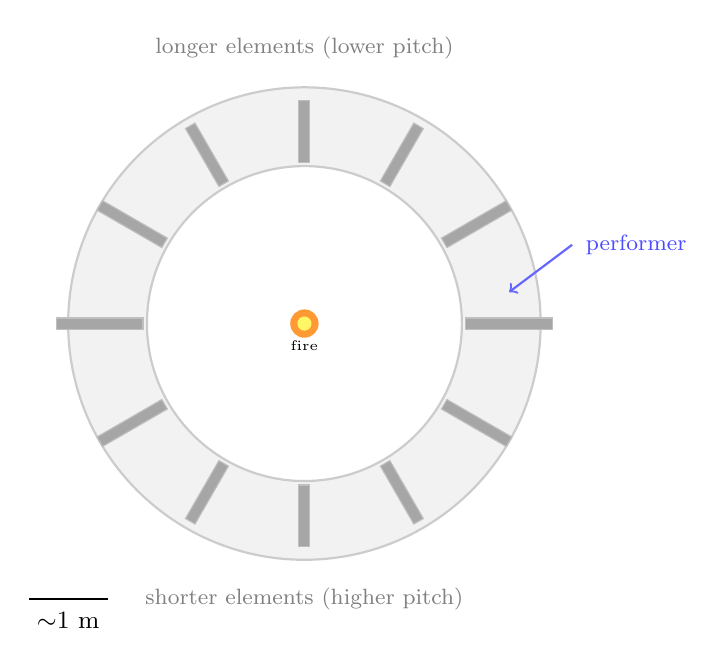
\begin{tikzpicture}[scale=1.0]

% Draw main ring outline
\draw[thick, gray!40, fill=gray!10] (0,0) circle (3.0cm);

% Draw inner ring outline
\draw[thick, gray!40, fill=white] (0,0) circle (2.0cm);

% Place 12 "stalagmite" elements around the ring, varying heights for pitch
% Each is a small rectangle at angle theta, pointing radially outward
\foreach \angle/\ht/\lbl in {
  0/1.1/A,
  30/0.95/B,
  60/0.85/C,
  90/0.78/D,
  120/0.85/E,
  150/0.95/F,
  180/1.1/G,
  210/0.95/H,
  240/0.85/I,
  270/0.78/J,
  300/0.85/K,
  330/0.95/L
}{
  \begin{scope}[rotate=\angle]
    \fill[gray!70] (2.05,-0.07) rectangle (2.05+\ht, 0.07);
    \draw[thin,gray!50] (2.05,-0.07) rectangle (2.05+\ht, 0.07);
  \end{scope}
}

% Central fire marker
\fill[orange!80] (0,0) circle (0.18cm);
\fill[yellow!60] (0,0) circle (0.09cm);
\node[font=\tiny] at (0,-0.28) {fire};

% Scale bar
\draw[thick] (-3.5,-3.5) -- (-2.5,-3.5);
\node[below, font=\small] at (-3.0,-3.55) {$\sim$1 m};

% Compass annotations
\node[font=\footnotesize, gray] at (0, 3.5) {longer elements (lower pitch)};
\node[font=\footnotesize, gray] at (0, -3.5) {shorter elements (higher pitch)};

% Arrow for "performer position"
\draw[->, thick, blue!60] (3.4, 1.0) -- (2.6, 0.4);
\node[right, font=\footnotesize, blue!70] at (3.45, 1.0) {performer};

\end{tikzpicture}
\caption{Schematic plan view of a hypothetical Bruniquel lithophone ring (Structure~1, $\varnothing \approx 6.7$~m not to scale). Shaded rectangles represent stalagmite elements of varying lengths arranged around the ring circumference. Longer elements (lower pitch) are shown at top and bottom; shorter elements (higher pitch) at the lateral positions, suggesting a hypothetical tonal layout. The central orange circle indicates the approximate position of fire remains as reported by \citet{Jaubert2016}. This diagram is entirely hypothetical and does not reflect measured fragment positions.}
\label{fig:ring}
\end{figure}

%------------------------------------------------------------------
\section{Proposed Experimental Protocol for Testing the Stone Piano Hypothesis}
%------------------------------------------------------------------

This appendix outlines a concrete experimental programme for evaluating the Stone Piano Hypothesis. The protocol is designed to be implementable with currently available techniques and equipment, using substitute speleothem materials where direct access to the Bruniquel samples is unavailable.

\subsection*{Phase 1: Acoustic characterization of calcite speleothem samples}

\textit{Materials.} Obtain 20--30 calcite stalagmite or stalactite fragments from non-heritage cave sites in the Périgord-Quercy limestone karst of southwestern France, with lengths spanning 30--80~cm and varying cross-sectional diameters. Document the mass, length, maximum and minimum diameters, and taper of each fragment.

\textit{Procedure.} Suspend each fragment from a thin nylon cord at its predicted nodal point (at $0.224L$ from one end for the fundamental free--free bending mode). Strike the fragment with three standardized implements: a river cobble of approximately 200~g, an antler billet of approximately 150~g, and a wooden mallet. Record acoustic output with a calibrated microphone at 48~kHz sample rate and 24-bit depth. Compute the fast Fourier transform (FFT) spectrum of each strike to identify fundamental frequency and overtone series. Measure $T_{60}$ for each mode from the spectral decay envelope.

\textit{Analysis.} Fit observed fundamental frequencies against equation~\eqref{eq:circular} with $E$ and $\rho$ as free parameters; report best-fit values and assess residuals. Evaluate whether the overtone ratios are consistent with the free--free beam prediction. Assess perceived pitch salience through forced-choice listener tests with naïve participants.

\subsection*{Phase 2: Morphometric analysis of Bruniquel fragments}

\textit{Materials.} If direct access to Bruniquel samples is unavailable, use existing three-dimensional photogrammetric or LiDAR models of the structures. If available, supplement with direct caliper and laser measurement of accessible fragments.

\textit{Procedure.} Measure the longest dimension (effective length) and the mean cross-sectional diameter of each identifiable ring-forming fragment. For tapered fragments, record both proximal and distal diameters and estimate the effective acoustic length.

\textit{Statistical analysis.} Test the null hypothesis that fragment lengths are drawn from a uniform or log-normal distribution consistent with random fracture. Apply a Kolmogorov--Smirnov goodness-of-fit test and a Hartigan dip test for multimodality. If multimodal clustering is detected, evaluate whether the cluster centroids are consistent with the harmonic length ratios given in Table~\ref{tab:ratios}.

\subsection*{Phase 3: Surface examination for percussion wear}

\textit{Materials.} A subset of Bruniquel fragments, or comparable experimentally percussion-used calcite fragments.

\textit{Procedure.} Clean fragment surfaces with deionized water and soft brushes. Examine under stereomicroscope at $\times 10$--$\times 50$ magnification. Image candidate percussion-damage zones with SEM at $\times 100$--$\times 2000$. Quantify surface roughness at percussion and non-percussion zones using three-dimensional profilometry. Apply micro-XRF to identify elemental signatures of percussive implement materials.

\textit{Controls.} Prepare experimental percussion samples by striking calcite fragments with cobble, antler, and bone implements at controlled forces and angles. Prepare taphonomic control samples by tumbling calcite fragments in sediment. Compare damage morphology to distinguish deliberate percussion from taphonomic damage.

\subsection*{Phase 4: Acoustic modeling of the Bruniquel chamber}

\textit{Materials.} Published geometric data from \citet{Jaubert2016}, supplemented if possible by detailed photogrammetric survey data.

\textit{Procedure.} Reconstruct the chamber geometry as a three-dimensional mesh. Assign surface absorption coefficients appropriate to bare limestone ($\alpha \approx 0.02$--$0.05$). Compute the room impulse response using an image source method or finite-difference time-domain (FDTD) simulation. Extract $T_{60}$ as a function of frequency and identify chamber resonance modes. Compute the sound pressure level distribution within the chamber for a point source at the ring position.

\textit{Deliverables.} A predicted spatial map of reverberation intensity within the Bruniquel chamber, with the positions of the stalagmite rings marked. Assessment of whether the ring positions coincide with acoustic antinodes or high-reverberation zones.

\end{document}

